\subsection*{Teil A: Achsensymmetrie (25 Minuten)}

\begin{merkbox}[Achsensymmetrie]
    Eine Figur ist \textbf{achsensymmetrisch}, wenn sie durch Spiegelung an einer Geraden (Symmetrieachse) auf sich selbst abgebildet wird.
\end{merkbox}

\begin{enumerate}[label=\arabic*.]

    \item \textbf{Zeichne die Spiegelpunkte ein und vervollständige die Figur:}

    \vspace{0.5cm}

    \begin{center}
        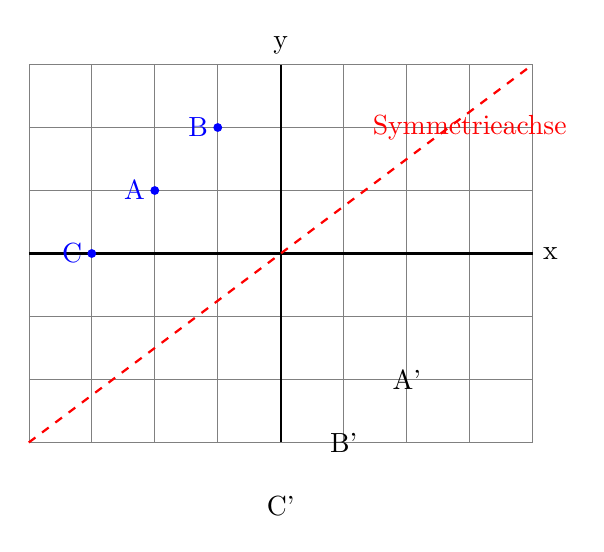
\begin{tikzpicture}[scale=0.8]
            % Koordinatensystem
            \draw[help lines] (-4,-3) grid (4,3);
            \draw[thick] (-4,0) -- (4,0) node[right] {x};
            \draw[thick] (0,-3) -- (0,3) node[above] {y};

            % Symmetrieachse
            \draw[thick, red, dashed] (-4,-3) -- (4,3);
            \node[red] at (3,2) {Symmetrieachse};

            % Gegebene Punkte
            \fill[blue] (-2,1) circle (2pt) node[left] {A};
            \fill[blue] (-1,2) circle (2pt) node[left] {B};
            \fill[blue] (-3,0) circle (2pt) node[left] {C};

            % Platz für Spiegelpunkte
            \node at (2,-2) {A'};
            \node at (1,-3) {B'};
            \node at (0,-4) {C'};
        \end{tikzpicture}
    \end{center}

    \vspace{1cm}

    \item \textbf{Bestimme alle Symmetrieachsen der folgenden Figuren:}

    \vspace{0.5cm}

    \begin{center}
        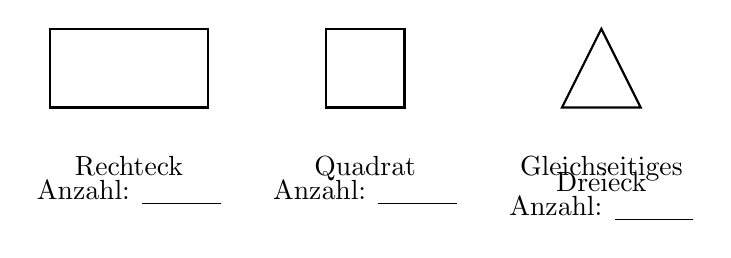
\begin{tikzpicture}
            % Rechteck
            \begin{scope}[xshift=-3cm]
                \draw[thick] (-1,-0.5) rectangle (1,0.5);
                \node[below] at (0,-1) {Rechteck};
                \node[below] at (0,-1.3) {Anzahl: \underline{\hspace{1cm}}};
            \end{scope}

            % Quadrat  
            \begin{scope}[xshift=0cm]
                \draw[thick] (-0.5,-0.5) rectangle (0.5,0.5);
                \node[below] at (0,-1) {Quadrat};
                \node[below] at (0,-1.3) {Anzahl: \underline{\hspace{1cm}}};
            \end{scope}

            % Gleichseitiges Dreieck
            \begin{scope}[xshift=3cm]
                \draw[thick] (0,0.5) -- (-0.5,-0.5) -- (0.5,-0.5) -- cycle;
                \node[below] at (0,-1) {Gleichseitiges};
                \node[below] at (0,-1.2) {Dreieck};
                \node[below] at (0,-1.5) {Anzahl: \underline{\hspace{1cm}}};
            \end{scope}
        \end{tikzpicture}
    \end{center}

    \vspace{1cm}

    \item \textbf{Konstruktion der Mittelsenkrechten:}

    Zeichne mit Zirkel und Lineal die Mittelsenkrechte der Strecke AB.

    \vspace{0.5cm}

    \begin{center}
        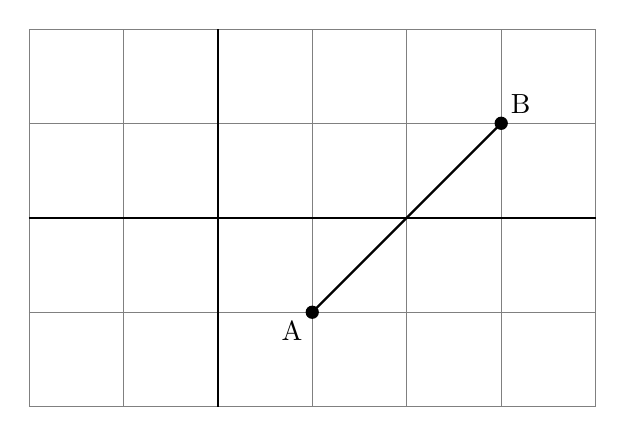
\begin{tikzpicture}[scale=1.2]
            % Koordinatensystem
            \draw[help lines] (-2,-2) grid (4,2);
            \draw[thick] (-2,0) -- (4,0);
            \draw[thick] (0,-2) -- (0,2);

            % Strecke AB
            \draw[thick] (1,-1) -- (3,1);
            \fill (1,-1) circle (2pt) node[below left] {A};
            \fill (3,1) circle (2pt) node[above right] {B};
        \end{tikzpicture}
    \end{center}

    \textit{Konstruktionsschritte:}
    \begin{enumerate}[label=\arabic*.]
        \item Zeichne um A einen Kreis (Radius > halbe Strecke AB)
        \item Zeichne um B einen Kreis mit \underline{\hspace{3cm}} Radius
        \item Verbinde die \underline{\hspace{3cm}} der beiden Kreise
    \end{enumerate}

\end{enumerate}